\chapter{Prometheus And Grafana}
\label{chap:prometheusAndGrafana}


\section{Technologies Used}
\begin{itemize}
    \item \textbf{Prometheus} is a monitoring system that collects and stores time-series metrics from various sources by scraping HTTP endpoints at regular intervals.
    \item \textbf{Node Exporter} is an agent that runs on your servers and exposes system-level metrics in a format Prometheus can scrape.
    \item \textbf{Grafana} is a visualization platform that queries Prometheus data and displays it through customizable dashboards with graphs and alerts.
    \item \textbf{Dashboard 1860} It shows real-time and historical data about CPU usage, memory consumption, disk I/O and space, network traffic, and system load.
\end{itemize}

\section{Executed Outputs}

\begin{figure}[htbp]
    \centering
    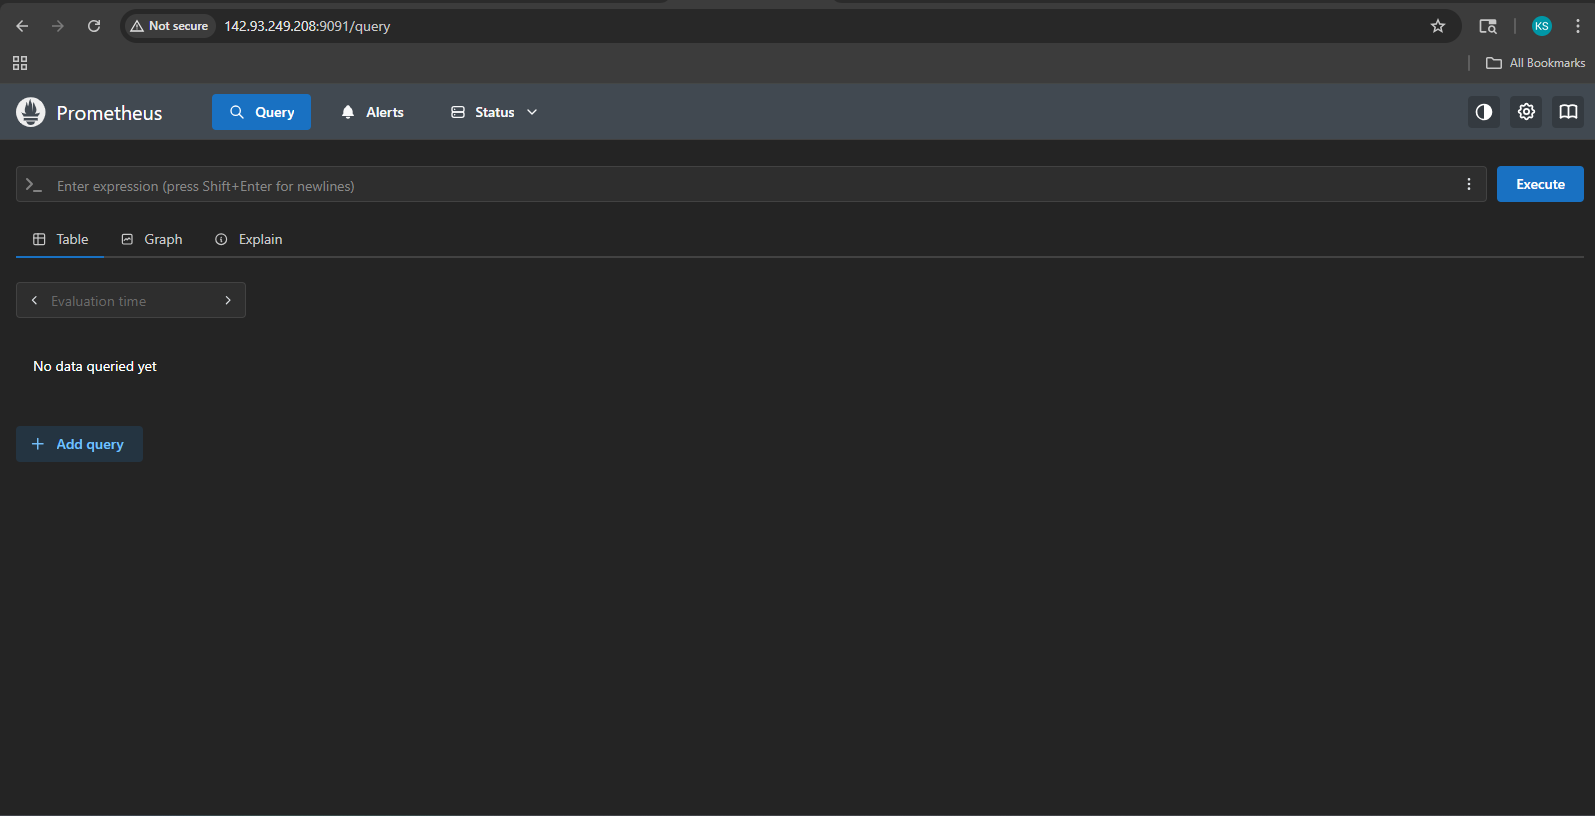
\includegraphics[width=0.8\textwidth]{png/PrometheusAndGrafana/prometheus-dashboard.png}
    \caption{Prometheus Dashboard Image - 1}
    \label{fig:prometheusDashboard-1}
\end{figure}

\begin{figure}[htbp]
    \centering
    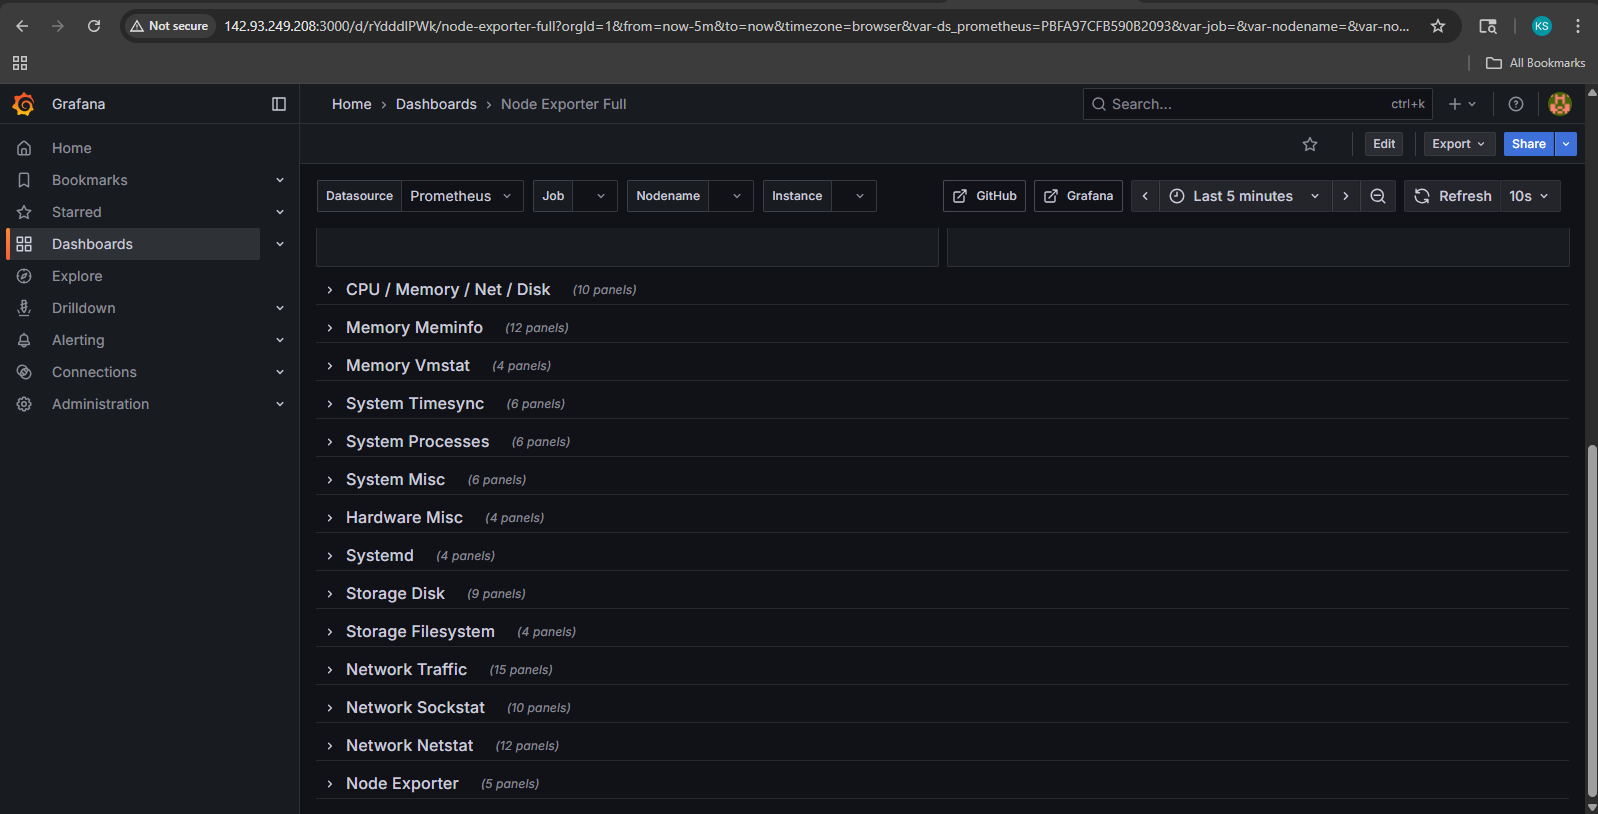
\includegraphics[width=0.8\textwidth]{png/PrometheusAndGrafana/prometheus-dashboard-2.png}
    \caption{Prometheus Dashboard Image - 2}
    \label{fig:prometheusDashboard-2}
\end{figure}

\begin{figure}[htbp]
    \centering
    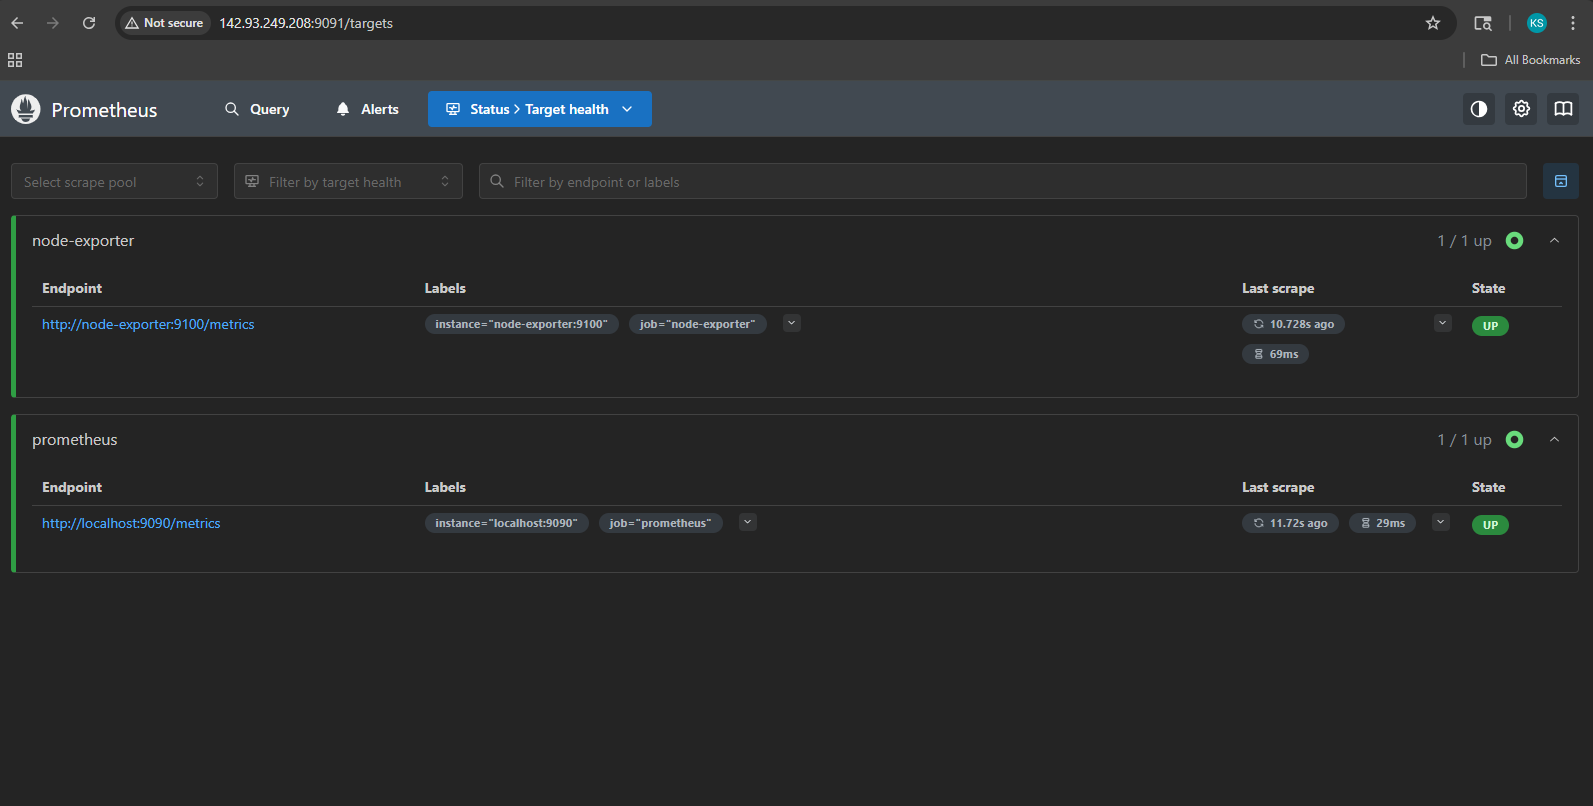
\includegraphics[width=0.8\textwidth]{png/PrometheusAndGrafana/prometheus-status.png}
    \caption{Prometheus Status Page}
    \label{fig:prometheusStatus}
\end{figure}

\begin{figure}[htbp]
    \centering
    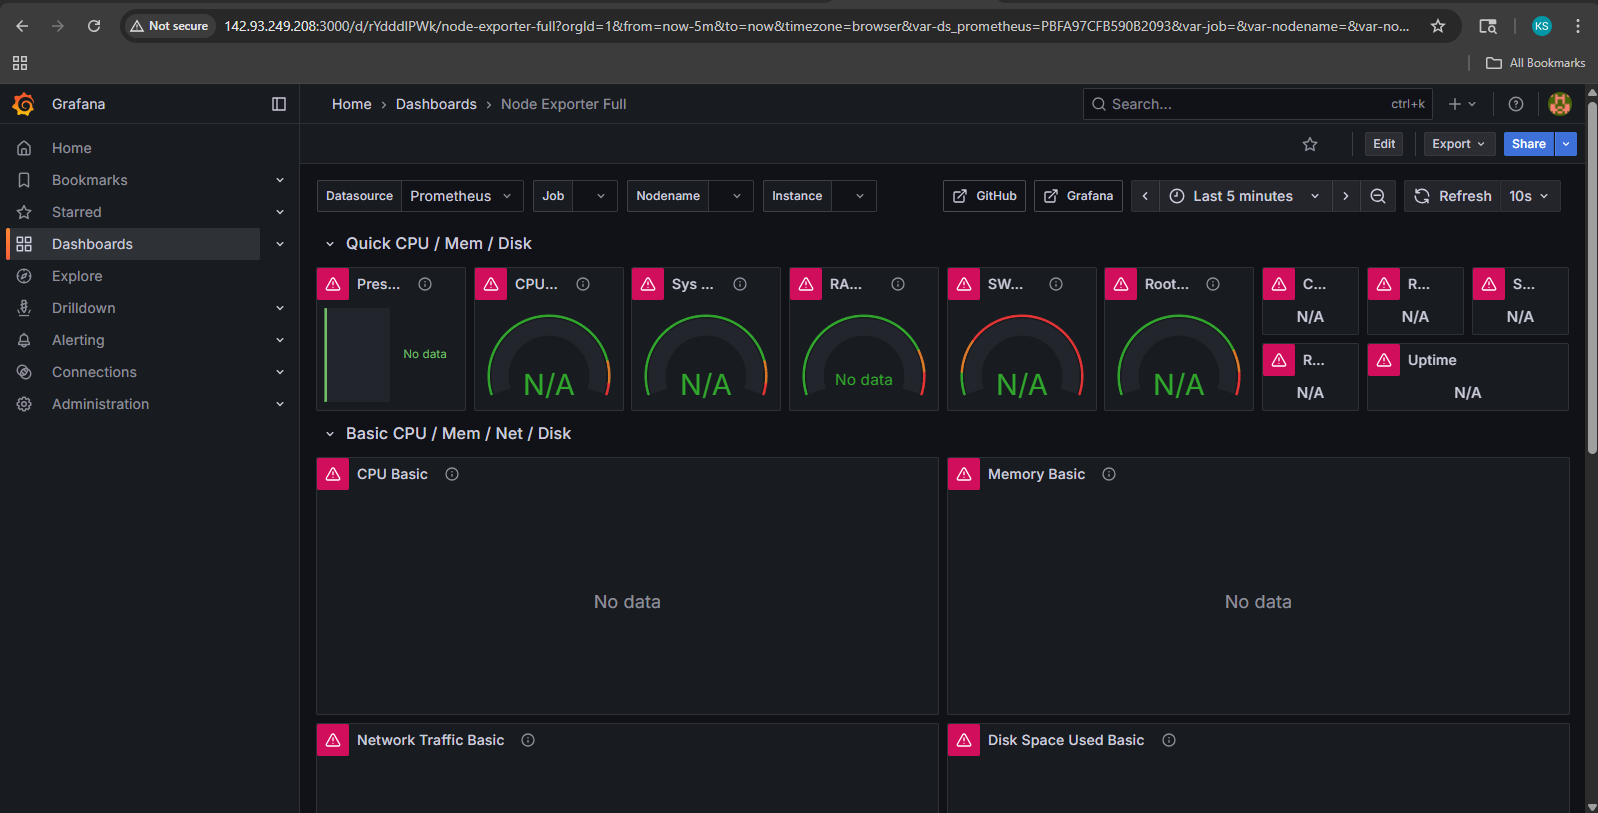
\includegraphics[width=0.8\textwidth]{png/PrometheusAndGrafana/grafana-dashboard.png}
    \caption{Grafana 1860 Dashboard}
    \label{fig:grafanaDashboard}
\end{figure}

\begin{figure}[htbp]
    \centering
    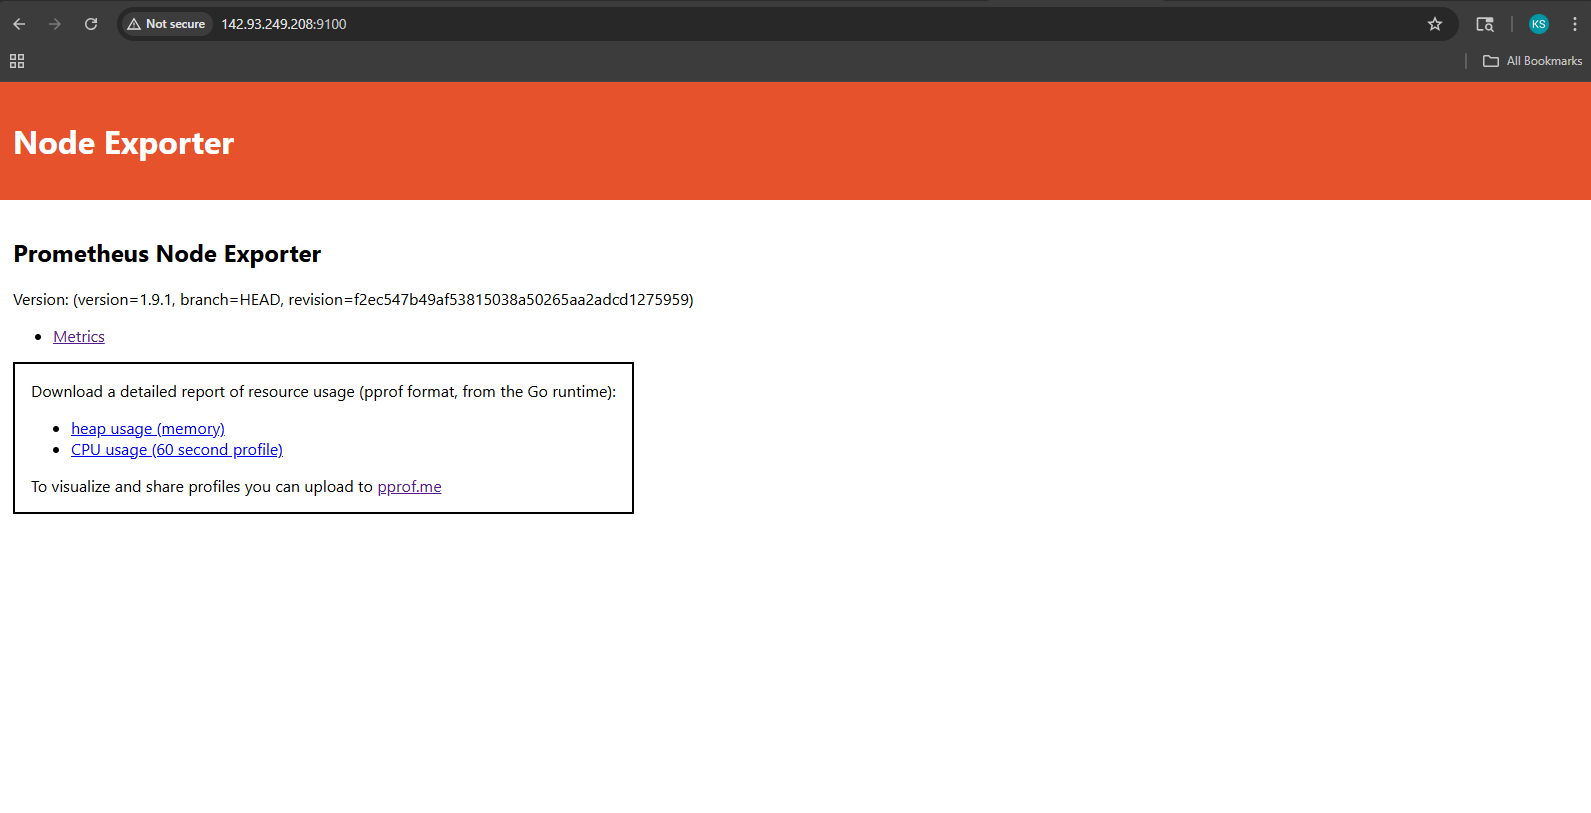
\includegraphics[width=0.8\textwidth]{png/PrometheusAndGrafana/node-exporter-home.png}
    \caption{Node Exporter Home}
    \label{fig:nodeExporterHome}
\end{figure}

